%
%intro
The stack implementation tests were mainly focused on the interactions established between the packages at play and the surrounding systems both lower-tiered and high-tiered.
%
\subsubsection{IO: Input/Output Package}
%
The IO package testing (figure \ref{fig:io-test}) consisted in the creation of a GPIO object with which one could simulate motor PWM outputs that would generate a file, through which one would simulate the IR sensor readings or motor pulse readings. The first GPIO test relied on a configuration of an object in OUTPUT\_PWM mode. With the latter test, it was possible to write three 32 bit integers to a binary file and observe the results with notepad++.
The second test hinged on reading from the forementioned binary file, expecting to retrieve the corresponding values. Should the latter be as expected the test could be considered a success.
%
\subsubsection{COM: Communications Package}
%
The COM package testing involved effectuating some experiments between the \gls{nvs} and the smartphone (using Bluetooth) and the former and the \gls{rvvs} (using RS232). These experiments will be performed in section \ref{sec:nvs-tests}.
%
\subsubsection{OS: Scheduler Package}
%
\subsubsection{MEM: Memory Structures Package}
%
\subsubsection{CLK: Timing Package}
%
The CLK package testing (figure \ref{fig:clk-test}) included the creation of a Timer object, associating it to a callback and proceed to verify if the callback was called at the specified time preemptively defined in the Config object configuration.
%
\begin{figure}[!ht]
\centering
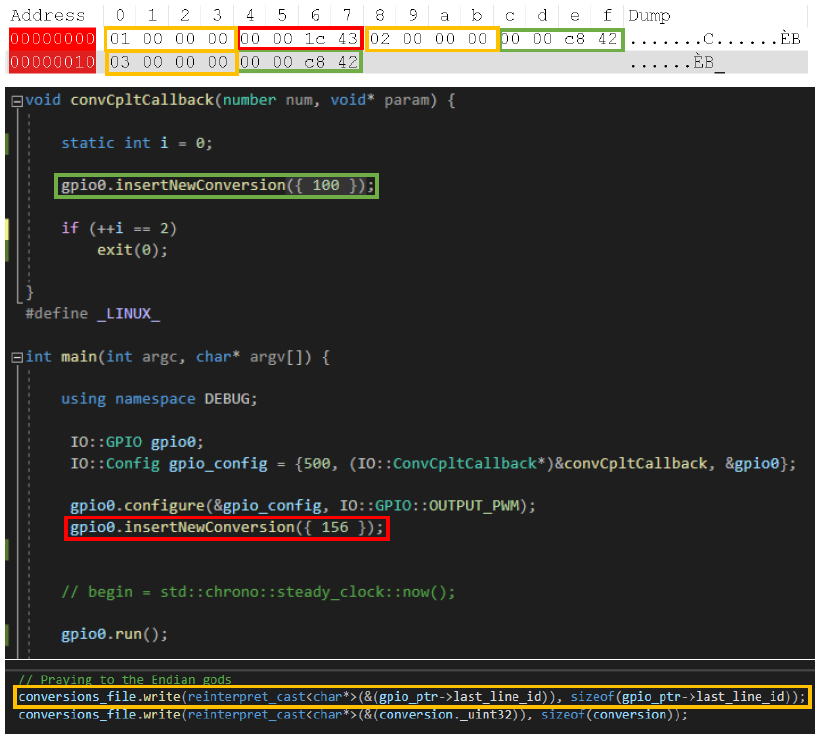
\includegraphics[width=0.8\textwidth]{img/IO-test.png}
\caption{\label{fig:io-test}IO package OUTPUT\_PMW mode tests}
\end{figure}
%
%
\begin{figure}[!ht]
\centering
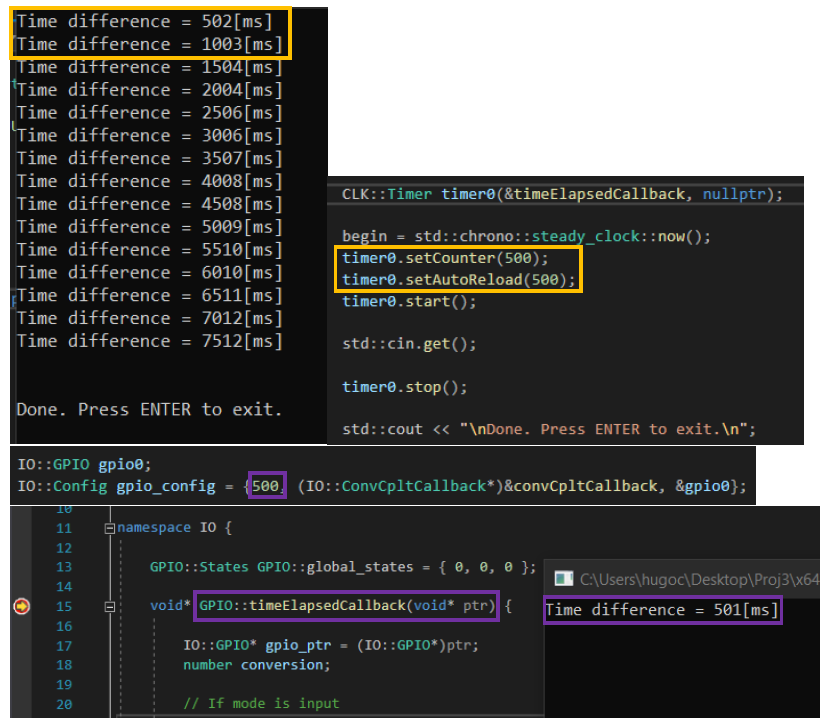
\includegraphics[width=0.8\textwidth]{img/CLK-test.png}
\caption{\label{fig:clk-test}CLK package tests}
\end{figure}
%